% Mid-project report, ACL style (same template as the proposal).
% Compile: pdflatex main && bibtex main && pdflatex main && pdflatex main
% Figures: python reports/mid/make_figures.py (from the repository root)
\documentclass[11pt]{article}

\usepackage[final]{acl}

\usepackage{times}
\usepackage{latexsym}
\usepackage[T1]{fontenc}
\usepackage[utf8]{inputenc}
\usepackage{microtype}
\usepackage{inconsolata}
\usepackage{amsmath}
\usepackage{amssymb}
\usepackage{booktabs}
\usepackage{tabularx}
\usepackage{enumitem}
\usepackage{graphicx}
\usepackage{tikz}
\usetikzlibrary{positioning,arrows.meta,fit}

\setlist{nosep,leftmargin=*}

\newcommand{\action}[1]{\texttt{#1}}
\newcommand{\seed}{S_i^{(0)}}

\title{When Does Graph Expansion Help? Measurement-Driven, Issue-Adaptive\\
Retrieval Routing for Repository-Level Code Localization\\[4pt]
\large Mid-Project Report}

\author{
  Naman Singhal \\
  2024114013 \\
  \And
  Yash More \\
  2024114004 \\
  \And
  Aaditya Bhatiya \\
  2023114012
}

\begin{document}
\maketitle

\begin{abstract}
We study when a cheap retrieval step after a first keyword search helps to
localize the code relevant to a repository-level issue, and whether simple
signals can predict it. This report covers the first four of our seven
stages. We built the full Phase~A pipeline on the 500 Python issues of
SWE-Explore (15 repositories): pre-fix snapshots, function-level chunks, a
BM25 seed, a typed repository graph, a frozen dense retriever, reciprocal-rank
fusion, three edge-typed graph expansions, and an evaluation harness checked
against SWE-Explore's released scorer. We then ran all six actions on all 500
issues at three line budgets. Three findings stand out. First, no action is
uniformly useful: every action except inheritance expansion helps 35--52\% of
issues and hurts another 35--49\%, and picking the best action per issue would
score 40\% above the best fixed action (fusion). Second, of the proposal's
five specific expectations only one holds (a hub as the top seed hit makes
expansion hurt), while the graph degree of the top seed hit turns out to be
the strongest signal overall. Third, one routing rule is stable across all
eight training folds: when the top hit is a call hub and the dense retriever
disagrees with BM25, follow call edges instead of fusing. The held-out
evaluation of the rule-based router (Stage~5) is next.
\end{abstract}

%======================================================================
\section{Introduction}
%======================================================================

Before a coding agent can fix an issue, it must find the code relevant to it.
This \emph{issue localization} step is retrieval under a hard budget: the
agent's context window is finite, so every retrieved chunk displaces another.
Retrieval-only methods (lexical BM25~\citep{robertson2009bm25} or dense
embeddings) are cheap but miss code that shares no words with the issue.
Graph-based agents such as LocAgent~\citep{chen2025locagent},
CoSIL~\citep{jiang2025cosil} and OrcaLoca~\citep{yu2025orcaloca} follow calls,
imports and inheritance, but the decision of when to expand is left to the
model's reasoning.

Our proposal asked two questions. \textbf{Phase~A:} under a fixed budget, how
much does each retrieval action (dense retrieval, fusion, or one-hop expansion
along one edge type) improve on a BM25 seed for each issue, and which cheap
signals predict when it helps? \textbf{Phase~B:} can those findings be turned
into an explicit, interpretable router that picks one action per issue, and
does it beat the best fixed action on held-out repositories?

\paragraph{Status.} Stages 1 to 4 of 7 are done (Table~\ref{tab:timeline}),
about a week ahead of the proposal's timeline: the data and pipeline, the
evaluation harness and dense retriever, the expansion actions and the full
Phase~A run, and the Phase~A analysis with a frozen rule procedure for the
Tier~1 router. Section~\ref{sec:built} describes what we built (after a recap and an
updated related-work section),
Section~\ref{sec:results} the results so far, Section~\ref{sec:obs} our
observations, Section~\ref{sec:dev} where we departed from the proposal, and
Section~\ref{sec:left} what is left.

%======================================================================
\section{Study Design (Recap)}
%======================================================================

\begin{figure*}[t]
\centering
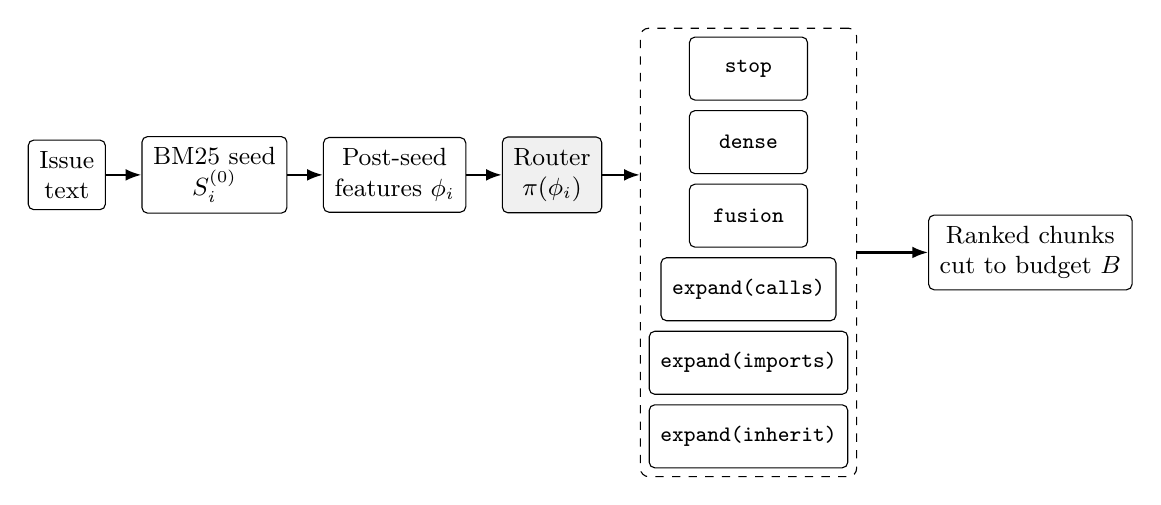
\begin{tikzpicture}[
  node distance=0.5cm and 0.45cm,
  box/.style={draw, rounded corners=2pt, align=center, font=\small,
              minimum height=0.8cm, inner sep=4pt},
  act/.style={box, font=\footnotesize\ttfamily, minimum width=1.5cm},
  arr/.style={-{Latex[length=2mm]}, thick}
]
  \node[box] (issue) {Issue\\text};
  \node[box, right=of issue] (bm25) {BM25 seed\\$\seed$};
  \node[box, right=of bm25] (feat) {Post-seed\\features $\phi_i$};
  \node[box, right=of feat, fill=gray!12] (router) {Router\\$\pi(\phi_i)$};

  \node[act, right=1.1cm of router, yshift=1.35cm] (a1) {stop};
  \node[act, below=0.12cm of a1] (a2) {dense};
  \node[act, below=0.12cm of a2] (a3) {fusion};
  \node[act, below=0.12cm of a3] (a4) {expand(calls)};
  \node[act, below=0.12cm of a4] (a5) {expand(imports)};
  \node[act, below=0.12cm of a5] (a6) {expand(inherit)};
  \node[draw, dashed, rounded corners=3pt, fit=(a1)(a6), inner sep=3pt] (acts) {};

  \node[box, right=0.9cm of acts] (out) {Ranked chunks\\cut to budget $B$};

  \draw[arr] (issue) -- (bm25);
  \draw[arr] (bm25) -- (feat);
  \draw[arr] (feat) -- (router);
  \draw[arr] (router) -- (acts.west |- router);
  \draw[arr] (acts) -- (out);
\end{tikzpicture}
\caption{Overview (unchanged from the proposal). Phase~A runs \emph{every}
action on every issue to measure its gain over the seed; Phase~B selects one
action per issue in advance from cheap features.}
\label{fig:overview}
\end{figure*}

For issue $i$ with text $q_i$ and pre-fix snapshot $R_i$, every system returns
ranked code chunks cut to a budget of $B$ lines ($B=300$ primary; 100 and 500
also reported). Holding $B$ fixed means no action can win by returning more
code. The gain of action $a$ over the seed is
\begin{equation}
  \Delta(i,a) = \mathrm{Score}\big(S_i^{(a)}\big) - \mathrm{Score}\big(\seed\big),
\end{equation}
with nDCG@300 on SWE-Explore core regions as the primary score. The six
actions are \action{stop} (the seed unchanged), \action{dense},
\action{fusion}, and \action{expand}$(e)$ for
$e \in \{\text{calls}, \text{imports/containment}, \text{inheritance}\}$
(Figure~\ref{fig:overview}).

%======================================================================
\section{Related Work (Updated)}
%======================================================================

\paragraph{Graph-based and agentic localization.} LocAgent~\citep{chen2025locagent},
CoSIL~\citep{jiang2025cosil} and OrcaLoca~\citep{yu2025orcaloca} let an LLM
search a repository graph; AutoCodeRover~\citep{zhang2024autocoderover} and
Agentless~\citep{xia2024agentless} localize with code search and hierarchical
narrowing; RepoGraph~\citep{ouyang2024repograph} and
CodexGraph~\citep{liu2024codexgraph} provide graph infrastructure. In all of
them, when to expand is decided inside the model's reasoning. We reuse
LocAgent's graph builder but make that decision explicit.

\paragraph{Retrievers.} Trained localization retrievers such as
SWERank~\citep{reddy2026swerank} and CoRet~\citep{fehr2025coret} are
complementary: we use only frozen models, here CodeRankEmbed, trained on the
CoRNStack corpus~\citep{suresh2025cornstack}.

\paragraph{Selective expansion and query performance prediction.} Since the
proposal we found the closest precedent in classic IR. Pseudo-relevance
feedback helps on average but hurts many queries, so
\citet{amati2004query} and \citet{cronen2004selective} apply it selectively,
predicting from the query and its first-pass results whether expansion will
help. Such predictors grew into query performance prediction, e.g.\ clarity
\citep{cronen2002predicting} and score-spread measures such as
NQC~\citep{shtok2012nqc}. Our post-seed features are signals of this kind;
our setting differs in that expansion is structural (along code edges), the
router chooses among several typed actions, and a fixed line budget makes
every addition displace something.

\paragraph{Adaptive routing.} Adaptive-RAG~\citep{jeong2024adaptiverag} routes
questions among retrieval strategies by predicted complexity;
AIRCoder~\citep{shi2026aircoder} adapts retrieval for code completion, where
the target location is known; SWE-Router~\citep{son2026swerouter} routes
between agent models; Repository Memory~\citep{wang2026repomemory} adds
history tools to LocAgent but leaves their use to the agent. None routes among
localization mechanisms with an explicit policy.

\paragraph{Evaluation.} SWE-Explore~\citep{zhang2026sweexplore} scores ranked
line regions against what successful agent trajectories read, using
recall, nDCG~\citep{jarvelin2002ndcg} and noise under a line budget, which
credits code read during diagnosis and not only the lines a patch edits.

%======================================================================
\section{What We Built (Stages 1--3)}
\label{sec:built}
%======================================================================

\paragraph{Data.} SWE-Explore~\citep{zhang2026sweexplore} has 848 issues. Its
records carry the ground truth (core and optional line regions read by
successful agent trajectories) but no issue text or commit, so we join them
with SWE-bench Verified~\citep{jimenez2024swebench, openai2024verified} and
SWE-bench Pro. An issue counts as Python if every file its fix touched is
\texttt{.py}. This gives \textbf{500 issues from 15 repositories} (410
Verified from 12 repositories, 90 Pro from 3). Django alone has 207 issues
(41\%), then sympy 66, ansible 40, scikit-learn 31, qutebrowser 30 and
matplotlib 29. Full clones were too slow on the campus link, so we fetch only
the 499 needed pre-fix commits at depth 1 and only their \texttt{.py} files
(170\,MB for all 15 repositories).

\paragraph{Chunks, seed and graph.} Each snapshot is split into function,
class and module chunks (median about 28k chunks per snapshot). Chunks never
overlap, and every non-blank line belongs to exactly one chunk. BM25 uses a
code-aware tokenizer that splits \texttt{snake\_case} and \texttt{camelCase}
but also keeps the whole identifier. The repository graph adapts LocAgent's
open-source builder (contains, imports, invokes and inherits edges) and maps
its nodes onto our chunks. We made it about 5 times faster on django and
checked it edge for edge against the original on five repositories. The
outputs were hand-checked on 10 issues (the Stage~1 checkpoint), and 104
issues re-built from scratch on a second machine came out identical.

\paragraph{Evaluation harness.} We vendored SWE-Explore's released scorer and
report its metrics, but use two corrected metrics as primary:
\begin{itemize}
  \item \emph{Clipped ground truth.} Agents often ran \texttt{sed -n 1,240p} on
  a 146-line file, and the benchmark stores the requested range, so the
  official recall counts lines that do not exist. We clip regions to the file.
  \item \emph{nDCG with a ground-truth ideal.} The SWE-Explore paper defines
  the ideal ranking from the ground-truth regions, but the released code
  normalizes by the best reordering of the regions the system itself returned.
  Under the code's version a list whose only core hit is at rank 1 scores 1.0:
  75 of the 500 BM25 seeds get a perfect official nDCG@300 while covering only
  14\% of the core lines. We implement the paper's definition, so finding more
  core code is rewarded (its correlation with recall is 0.55 against 0.42).
\end{itemize}
Perfect Recall@$B$ is region-level (every core region touched), as the
proposal's wording says, because requiring every core line is impossible:
chunks drop the blank lines between definitions. The harness passes
hand-computed golden examples (the Stage~2 checkpoint) and matches the
official scorer exactly wherever the definitions agree.

\paragraph{Dense retrieval and fusion.} We use CodeRankEmbed, a frozen
137M-parameter code bi-encoder~\citep{suresh2025cornstack}. Because most files
do not change between snapshots of a repository, we embed each distinct chunk
once: 500 snapshots collapse to about 476k distinct chunks, embedded in about
25 minutes on one RTX 2080 Ti. Fusion is reciprocal-rank
fusion~\citep{cormack2009rrf}, $\sum 1/(k + \mathrm{rank})$, with $k=100$
chosen on dev (dev nDCG@300 rises from 0.137 at $k=5$ to 0.161 at $k=60$ and
0.162 at $k=100$).

\paragraph{Graph expansion.} As proposed, the top $k=10$ seed chunks are
parents; each depth-1 neighbour $n$ along the edge group gets
$s_e(n) = \max\big(s(n), \lambda \max_{p} s(p)\big)$ on min-max normalized
BM25 scores, the merged list is re-sorted and cut to $B$. With no neighbours
an expansion equals \action{stop} exactly. We tuned $\lambda$ and the edge
direction (outgoing only, or both directions) on dev
(Table~\ref{tab:tuning}). Calls and imports work best with
$\lambda = 0.99$ and both directions, which in effect places a seed hit's
callers and callees right after it. Inheritance edges are rare (0.28 per top
hit on average), so \action{expand(inherit)} changes nDCG on only 5\% of
issues.

\begin{table}[t]
\centering
\small
\setlength{\tabcolsep}{4pt}
\begin{tabular}{@{}lcccc@{}}
\toprule
Action & Dir. & $\lambda$ & dev nDCG & Gain \\
\midrule
\action{expand(calls)}   & both & 0.99 & 0.148 & $+0.029$ \\
\action{expand(imports)} & both & 0.99 & 0.134 & $+0.014$ \\
\action{expand(inherit)} & out  & 0.7  & 0.119 & $\phantom{+}0.000$ \\
\bottomrule
\end{tabular}
\caption{Expansion settings tuned on the 56 dev issues (grid
$\lambda \in \{0.5,\dots,0.99\}$ $\times$ direction); nDCG@300 and gain over
\action{stop} (0.119) on dev.}
\label{tab:tuning}
\end{table}

\paragraph{Splits.} With 15 repositories and django at 41\%, a single
train/dev/test split is not viable, so we use the proposal's fallback: a fixed
dev set (xarray, pytest, openlibrary; 56 issues, used only for tuning) plus
leave-one-repository-out over the rest, with the five smallest repositories
(29 issues) sharing one fold: 8 folds, 444 issues.

\paragraph{Post-seed features.} Computed from the issue text, the seed, the
graph and the dense scores only; nothing reads the patch or the ground truth.
They follow the proposal's list: traceback present (13\% of issues), the issue
names a \texttt{.py} path (36\%) or an existing repository file (18\%), number
of code identifiers that name a chunk (mean 5.2), a pasted environment dump
(8\%), issue length, BM25 score margins (top-1 and top-$k$), number of
distinct files in the seed top-10 (mean 5.8), graph degree of the top seed hit
(mean 19.8; per edge group as well), and BM25/dense top-10 overlap.

%======================================================================
\section{Results So Far (Phase A and Stage 4)}
\label{sec:results}
%======================================================================

All six actions were run on all 500 issues at $B \in \{100, 300, 500\}$ (9,000
scored rankings). Intervals are 95\% repository-clustered bootstrap
intervals: we resample whole repositories, since issues of one repository are
not independent.

\subsection{Fixed actions and the oracle}

\begin{table*}[t]
\centering
\small
\begin{tabular}{@{}l ccc ccc c c ccc@{}}
\toprule
 & \multicolumn{3}{c}{nDCG@$B$ (primary)} & \multicolumn{3}{c}{Line recall@$B$} & Perfect & Noise & \multicolumn{3}{c}{File recall@$B$ (Verified)} \\
\cmidrule(lr){2-4}\cmidrule(lr){5-7}\cmidrule(lr){10-12}
Action & 100 & 300 & 500 & 100 & 300 & 500 & @300 & @300 & 100 & 300 & 500 \\
\midrule
\action{stop} (BM25 seed) & .264 & .172 & .144 & .063 & .120 & .154 & .134 & .529 & .526 & .628 & .689 \\
\action{expand(inherit)}  & .264 & .172 & .144 & .063 & .120 & .155 & .132 & .528 & .534 & .638 & .700 \\
\action{expand(imports)}  & .263 & .170 & .143 & .064 & .131 & .170 & .132 & .517 & .471 & .596 & .648 \\
\action{expand(calls)}    & \textbf{.280} & .178 & .146 & .067 & .127 & .158 & .122 & .542 & .557 & .646 & .701 \\
\action{dense}            & .213 & .152 & .128 & .060 & .128 & .164 & \textbf{.170} & .524 & .555 & .676 & .737 \\
\action{fusion}           & .268 & \textbf{.184} & \textbf{.156} & \textbf{.068} & \textbf{.136} & \textbf{.182} & .160 & \textbf{.476} & \textbf{.557} & \textbf{.706} & \textbf{.770} \\
\midrule
Per-issue oracle (nDCG) & .392 & .258 & .212 & & & & & & & & \\
\bottomrule
\end{tabular}
\caption{Phase~A means over 500 issues (file recall: the 410 SWE-bench Verified
issues, against the files the developer patch edits). Perfect = every core
region touched; Noise = share of returned regions touching neither core nor
optional context (lower is better). The best fixed action depends on the
budget: \action{expand(calls)} at $B=100$, \action{fusion} at 300 and 500.}
\label{tab:main}
\end{table*}

\begin{figure}[t]
\centering
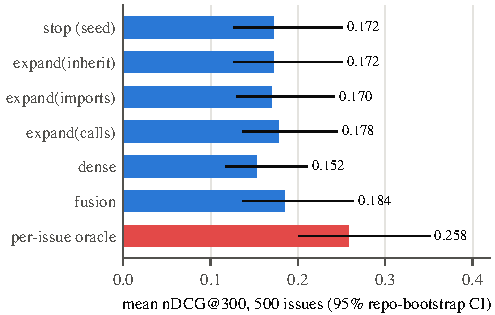
\includegraphics[width=\columnwidth]{figures/fixed_vs_oracle.pdf}
\caption{Mean nDCG@300 of each fixed action and of the per-issue oracle. The
wide intervals reflect how much the absolute level varies between
repositories; differences between actions are paired per issue and much
tighter (see the text).}
\label{fig:fixed}
\end{figure}

Table~\ref{tab:main} and Figure~\ref{fig:fixed} give the means. On average,
only fusion reliably beats the seed at $B=300$ (gain $+0.012$,
$[+0.002, +0.031]$), and only dense is reliably worse ($-0.020$,
$[-0.047, -0.006]$). No graph expansion moves the average at $B=300$:
\action{expand(calls)} $+0.006$ $[-0.009, +0.013]$, \action{expand(imports)}
$-0.002$, \action{expand(inherit)} $+0.000$. At the tightest budget, however,
\action{expand(calls)} is the best fixed action. The same ordering holds on
the SWE-bench file-level metric, where fusion lifts the share of patched files
returned at $B=300$ from 0.628 to 0.706.

\subsection{Gains are issue-dependent}

\begin{figure}[t]
\centering
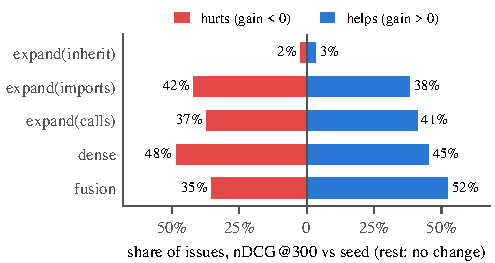
\includegraphics[width=\columnwidth]{figures/helps_hurts.pdf}
\caption{Share of issues each action helps or hurts compared with the seed
(nDCG@300, 500 issues).}
\label{fig:helps}
\end{figure}

The averages hide large per-issue effects (Figure~\ref{fig:helps}). Every
action except \action{expand(inherit)} helps 35--52\% of issues and hurts
another 35--49\%. The per-issue oracle scores 0.258 against fusion's 0.184,
40\% higher, and the action it picks is spread evenly: \action{stop} 17\%,
\action{expand(imports)} 20\%, \action{expand(calls)} 19\%, \action{dense}
22\%, \action{fusion} 21\%. No single action dominates, which is the premise
of the router. The picture is the same outside the dev repositories (444
issues: fusion 0.187, oracle 0.262).

\subsection{The proposal's expectations}

\begin{table}[t]
\centering
\small
\setlength{\tabcolsep}{4pt}
\begin{tabularx}{\columnwidth}{@{}X r@{}}
\toprule
Expectation, and measured gain over \action{stop} & Holds? \\
\midrule
\textbf{Traceback $\rightarrow$ \action{expand(calls)} helps.} & no \\
\multicolumn{2}{@{}p{\columnwidth}@{}}{\footnotesize with: $+.009$ $[-.015, +.034]$ ($n$=66); without: $+.005$} \\
\addlinespace
\textbf{Names target file $\rightarrow$ expansion adds noise.} & opposite \\
\multicolumn{2}{@{}p{\columnwidth}@{}}{\footnotesize calls $+.011$ $[-.002, +.016]$; imports $+.013$ $[-.001, +.029]$} \\
\addlinespace
\textbf{Hub top hit $\rightarrow$ expansion floods budget.} & yes \\
\multicolumn{2}{@{}p{\columnwidth}@{}}{\footnotesize calls, degree $>10$: $-.014$ $[-.036, +.001]$; $\leq 4$: $+.017$ $[+.009, +.031]$} \\
\addlinespace
\textbf{BM25/dense disagree $\rightarrow$ \action{fusion}.} & no \\
\multicolumn{2}{@{}p{\columnwidth}@{}}{\footnotesize fusion, disagree: $+.014$ $[-.003, +.048]$; agree: $+.012$} \\
\addlinespace
\textbf{Concentrated seed $\rightarrow$ \action{stop}.} & no \\
\multicolumn{2}{@{}p{\columnwidth}@{}}{\footnotesize no difference across score-margin bins} \\
\bottomrule
\end{tabularx}
\caption{The proposal's expectations, checked one feature at a time (gain
over \action{stop}, 95\% repository-bootstrap intervals).}
\label{tab:hyp}
\end{table}

Table~\ref{tab:hyp} checks the five expectations stated in the proposal. Only
the hub expectation holds. When the issue names the target file, expansion
helps slightly more, not less: the seed is right more often there (0.184 vs
0.169), and its neighbours are then relevant too. The proposal accepted that
Phase~A might be a partly negative result, and on these expectations it is.

\subsection{Signature table and the top-hit degree}

\begin{figure}[t]
\centering
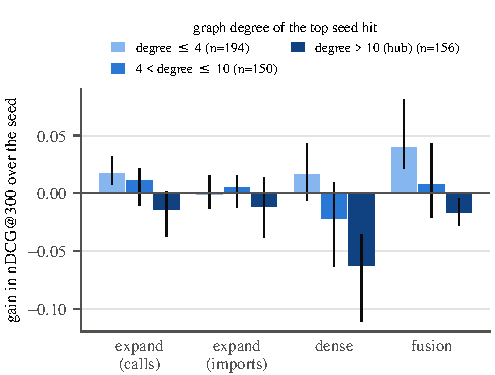
\includegraphics[width=\columnwidth]{figures/degree_effect.pdf}
\caption{Gain over the seed by the graph degree of the top seed hit (thirds of
the 500 issues), with 95\% repository-bootstrap intervals.}
\label{fig:degree}
\end{figure}

The signature table bins every feature (booleans by value, numbers into
thirds) and gives each action's mean gain, interval and help/hurt shares for
every bin and every pair of bins of two features (4,070 rows). Among cells
with at least 20 issues from at least 3 repositories, 46 of 205 single-feature
cells have an interval that excludes zero, against about 10 expected by
chance; for pairs it is 668 of 3,525 against about 176. The structure is real,
though any single cell may be a chance one.

The strongest signal is the graph degree of the top seed hit, and it matters
for every action, not only for expansion (Figure~\ref{fig:degree}). When the
top hit is a hub (degree $>10$), dense loses $0.062$ $[-0.110, -0.036]$ and
fusion $0.017$; when it is poorly connected (degree $\leq 4$), fusion gains
$0.040$ $[+0.022, +0.080]$ and \action{expand(calls)} $0.017$. Our reading is
that BM25 lands on a central, well-connected definition when the issue names
the right code, and then any change hurts.

\subsection{Tier 1 rules}

To keep the Stage~5 test honest, the Tier~1 rules come from a procedure fixed
before any held-out scoring rather than being written by hand after reading
the table (which would use the test repositories). On the training issues:
(1)~the default is the best fixed action; (2)~candidate conditions are every
feature bin and every pair of bins, with bin edges from the training issues;
(3)~rules are added greedily, each taking the condition and action with the
largest total gain over the default among those with at least 20 issues from
at least 3 repositories and a positive one-sided 95\% repository-bootstrap
lower bound; at most 5 rules of at most 2 conditions; (4)~an issue takes the
first matching rule, else the default.

\begin{table*}[t]
\centering
\small
\begin{tabularx}{\textwidth}{@{}c X l r r@{}}
\toprule
\# & If & Then & $n$ & Gain \\
\midrule
1 & top hit has $>7$ call edges and BM25/dense overlap $\leq 0.2$ & \action{expand(calls)} & 64 & $+.053$ \\
2 & names a \texttt{.py} path and top-hit degree in $(4, 10]$ & \action{expand(imports)} & 46 & $+.045$ \\
3 & seed spans $\leq 5$ files and top-hit degree $>10$ & \action{stop}$^\ast$ & 62 & $+.026$ \\
4 & Verified issue and top hit has inheritance edges & \action{expand(imports)} & 33 & $+.021$ \\
5 & top-$k$ margin in $(.15,.25]$ and overlap $>0.4$ & \action{dense} & 22 & $+.028$ \\
\midrule
 & otherwise & \action{fusion} & & \\
\bottomrule
\end{tabularx}
\caption{Rules found by the procedure on all 500 issues (descriptive). Gain
is nDCG@300 over the default (fusion) on the issues the rule covers.
$^\ast$Selected as \action{expand(inherit)}, which is in effect \action{stop}.}
\label{tab:rules}
\end{table*}

Table~\ref{tab:rules} lists the rules the procedure finds on all 500 issues.
In-sample this router scores 0.201 against fusion's 0.184, closing about 23\%
of the gap to the oracle; that number is optimistic because the rules were
selected on the same issues. We also fit the procedure on each fold's training
set (without scoring the held-out issues). \textbf{Rule~1 is found in all 8
folds}; every other rule appears in at most 4, with lower bounds close to
zero. On rule~1's 64 issues (10 repositories) the seed scores 0.202,
\action{expand(calls)} 0.213, fusion 0.161 and dense 0.121: when the top hit
is a call hub and dense disagrees with BM25, dense is wrong, fusion inherits
its mistakes, and the right move is to keep the seed and follow its call
edges. This reverses the proposal's guess that disagreement calls for fusion.

%======================================================================
\section{Observations}
\label{sec:obs}
%======================================================================

\begin{itemize}
  \item \textbf{The router has room, but the signals are weak.} The oracle gap
  is large (+40\%), but single features shift gains by only about 0.01 to 0.06,
  and most rules beyond the first are unstable. We expect the held-out router
  to close a small part of the gap, driven mostly by rule~1.
  \item \textbf{Ground truth caps every method.} SWE-Explore core regions are
  often whole files (median 1,160 core lines per issue; only 12.6\% of issues
  have 300 or fewer). Even a perfect ranker reaches only 39.5\% line recall at
  $B=300$ on average, which is why absolute recall values are low and why we
  use nDCG with a ground-truth ideal as the primary metric.
  \item \textbf{Repositories differ a lot.} The sign of a gain often flips
  between repositories (\action{expand(calls)}: matplotlib $+0.032$,
  scikit-learn $-0.046$; fusion: xarray $+0.112$, pylint $-0.046$). Pro issues,
  written in a templated style, gain more from every action (fusion $+0.028$ vs
  $+0.009$ on Verified).
  \item \textbf{Dev tuning transfers only partly.} \action{expand(calls)} gains
  $+0.029$ on dev but $+0.003$ outside it. Three dev repositories (56 issues)
  are a small tuning set.
  \item \textbf{Expansion is cheap but hubs are costly.} All actions take
  milliseconds per issue once the indexes exist. \action{expand(calls)} scores
  a median of 41 neighbours but up to 1,923 around a hub, which is the flooding
  the proposal expected.
  \item \textbf{Released metrics need care.} The official nDCG would reward an
  action that returns one tiny core hit at rank 1; reporting it as the headline
  would have hidden coverage differences between actions.
\end{itemize}

%======================================================================
\section{Departures from the Proposal}
\label{sec:dev}
%======================================================================

\begin{table}[t]
\centering
\small
\begin{tabularx}{\columnwidth}{@{}l X@{}}
\toprule
Item & What changed and why \\
\midrule
Splits & Leave-one-repository-out (the proposal's fallback): only 15 repositories. \\
Graph builder & Python's \texttt{ast} (as in LocAgent), not tree-sitter. \\
Primary nDCG & The paper's ground-truth ideal, on clipped regions; official scores also reported. \\
Perfect Recall & Region-level; the line-level version is unreachable by construction. \\
Dense model & One candidate (CodeRankEmbed), so no model selection on dev. \\
Edge direction & Tuned on dev per edge group ("both" for calls and imports). \\
Tier 1 rules & Produced by a fixed procedure per fold instead of written by hand, to avoid leakage. \\
Query & Not cleaned; instead a feature flags pasted environment dumps. \\
Schedule & Phase~A launched Oct 19, a day late; Stage~4 finished a week early. \\
\bottomrule
\end{tabularx}
\caption{Changes relative to the proposal.}
\label{tab:dev}
\end{table}

Table~\ref{tab:dev} lists every place where we departed from the proposal.
None changes the research questions; most follow the proposal's own fallbacks
or make the evaluation stricter.

%======================================================================
\section{What Is Left}
\label{sec:left}
%======================================================================

\begin{table*}[t]
\centering
\small
\begin{tabularx}{\textwidth}{@{}l l X l@{}}
\toprule
\textbf{Stage} & \textbf{Planned} & \textbf{Work} & \textbf{Status} \\
\midrule
1 & Oct 1--7   & Data, snapshots, chunking, BM25, graph builder & Done (10-issue hand-check) \\
2 & Oct 8--14  & Evaluation harness, dense retriever, fusion, splits; related work & Done (golden examples match) \\
3 & Oct 15--18 & Expansion actions, dev tuning, features; launch Phase~A & Done (Phase~A ran Oct 19) \\
4 & Oct 26--Nov 1 & Phase~A analysis, signature table, Tier~1 rules & Done early (Oct 19) \\
5 & Nov 2--8   & Tier~1 evaluation on held-out repositories; Tier~2 if on schedule & Next \\
6 & Nov 9--15  & Experiments frozen Nov 10; figures and write-up & To do \\
7 & Nov 16--20 & Revision and submission & To do \\
\bottomrule
\end{tabularx}
\caption{Progress against the proposal's timeline.}
\label{tab:timeline}
\end{table*}

\paragraph{Stage 5: held-out evaluation.} For each of the 8 folds, fit the
rule procedure on the other folds plus dev and route the held-out
repository's issues. We will report the router against the seed, the best
fixed action and the oracle, the share of the gap it closes,
\begin{equation}
  \mathrm{GapClosed}(\pi) =
  \frac{\mathrm{Score}(\pi) - \mathrm{Score}(\text{fixed})}
       {\mathrm{Score}(\text{oracle}) - \mathrm{Score}(\text{fixed})},
\end{equation}
repository-clustered intervals and paired per-issue comparisons, breakdowns by
repository and by whether the issue names a target file, cost (retrieval calls,
graph nodes visited, time), and the same at $B=100$ and 500 and on the
file-level metric. We also plan to report, as a secondary analysis declared before any
held-out result exists, the same router cut after its first rule, to test
whether the less stable rules add anything on unseen repositories.

\paragraph{Tier 2 (stretch).} The proposal allows a lightweight classifier
(logistic regression or a shallow tree) only if Tier~1 is evaluated by
November~1. Since we are ahead of schedule, it is within reach, using the same features
and folds, labels $\arg\max_a \Delta(i,a)$ and ties broken toward the
cheaper action.

\paragraph{Stages 6 and 7.} Freeze experiments on November~10, then write the
final report: the Phase~A signature table as a result in its own right, the
router results, and the limitations below.

\paragraph{Risks and limitations.} Fifteen repositories, one of them 41\% of
the data, make every interval wide and the leave-one-out folds unequal. The
signal for routing is weak, so the router may not beat fusion on held-out
repositories; the Phase~A table then stands as a conditional, partly negative
result, as the proposal anticipated. Our evaluation uses the reading-based
ground truth of SWE-Explore and file-level SWE-bench recall only; we do not
measure downstream repair.

\bibliography{references}

\end{document}
